\indent En lo que sigue, mostraremos buenos y malos casos para nuestro algoritmo, y a su vez, daremos el tiempo estimado 
seg\'un la complejidad del algoritmo calculada anteriormente.\\

Luego de varios experimentos, pudimos llegar a la conclusi\'on que uno de los tipos de casos que resulta m\'as beneficioso para nuestro algoritmo, dado que nuestro algoritmo es un BFS el cual va viendo todos los \textbf{caminos encuentra el camino m\'inimo m\'as r\'apido y corta la ejecuci\'on o ve que no puede romper la cantidad de paredes necesarias para avanzar por el camino en el inicio de cada camino posible}.\\

Un grafo que simplifica lo dicho es el siguiente:

\vspace*{0.3cm} \vspace*{0.3cm}
  \begin{center}
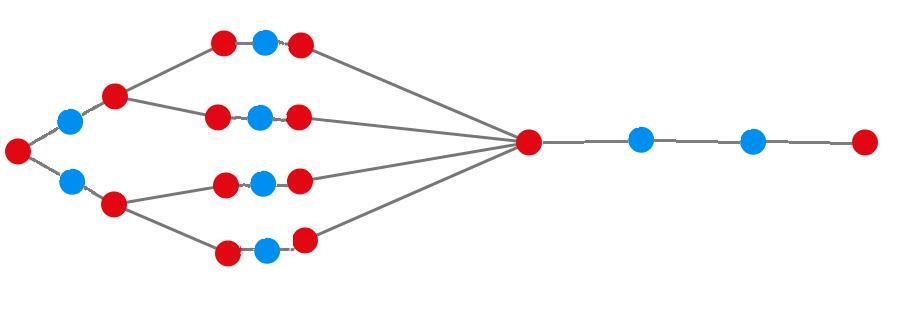
\includegraphics[scale=0.65]{./EJ1/ej1grafomejorcaso.jpeg}
{$Ejemplo Grafo$ \ 1.1 - $Mejor$ $Caso$}
  \end{center}
  \vspace*{0.3cm}


Para una mayor observaci\'on desarrollamos el siguiente gr\'afico con las instancias:\\

\vspace*{0.3cm} \vspace*{0.3cm}
  \begin{center}
 %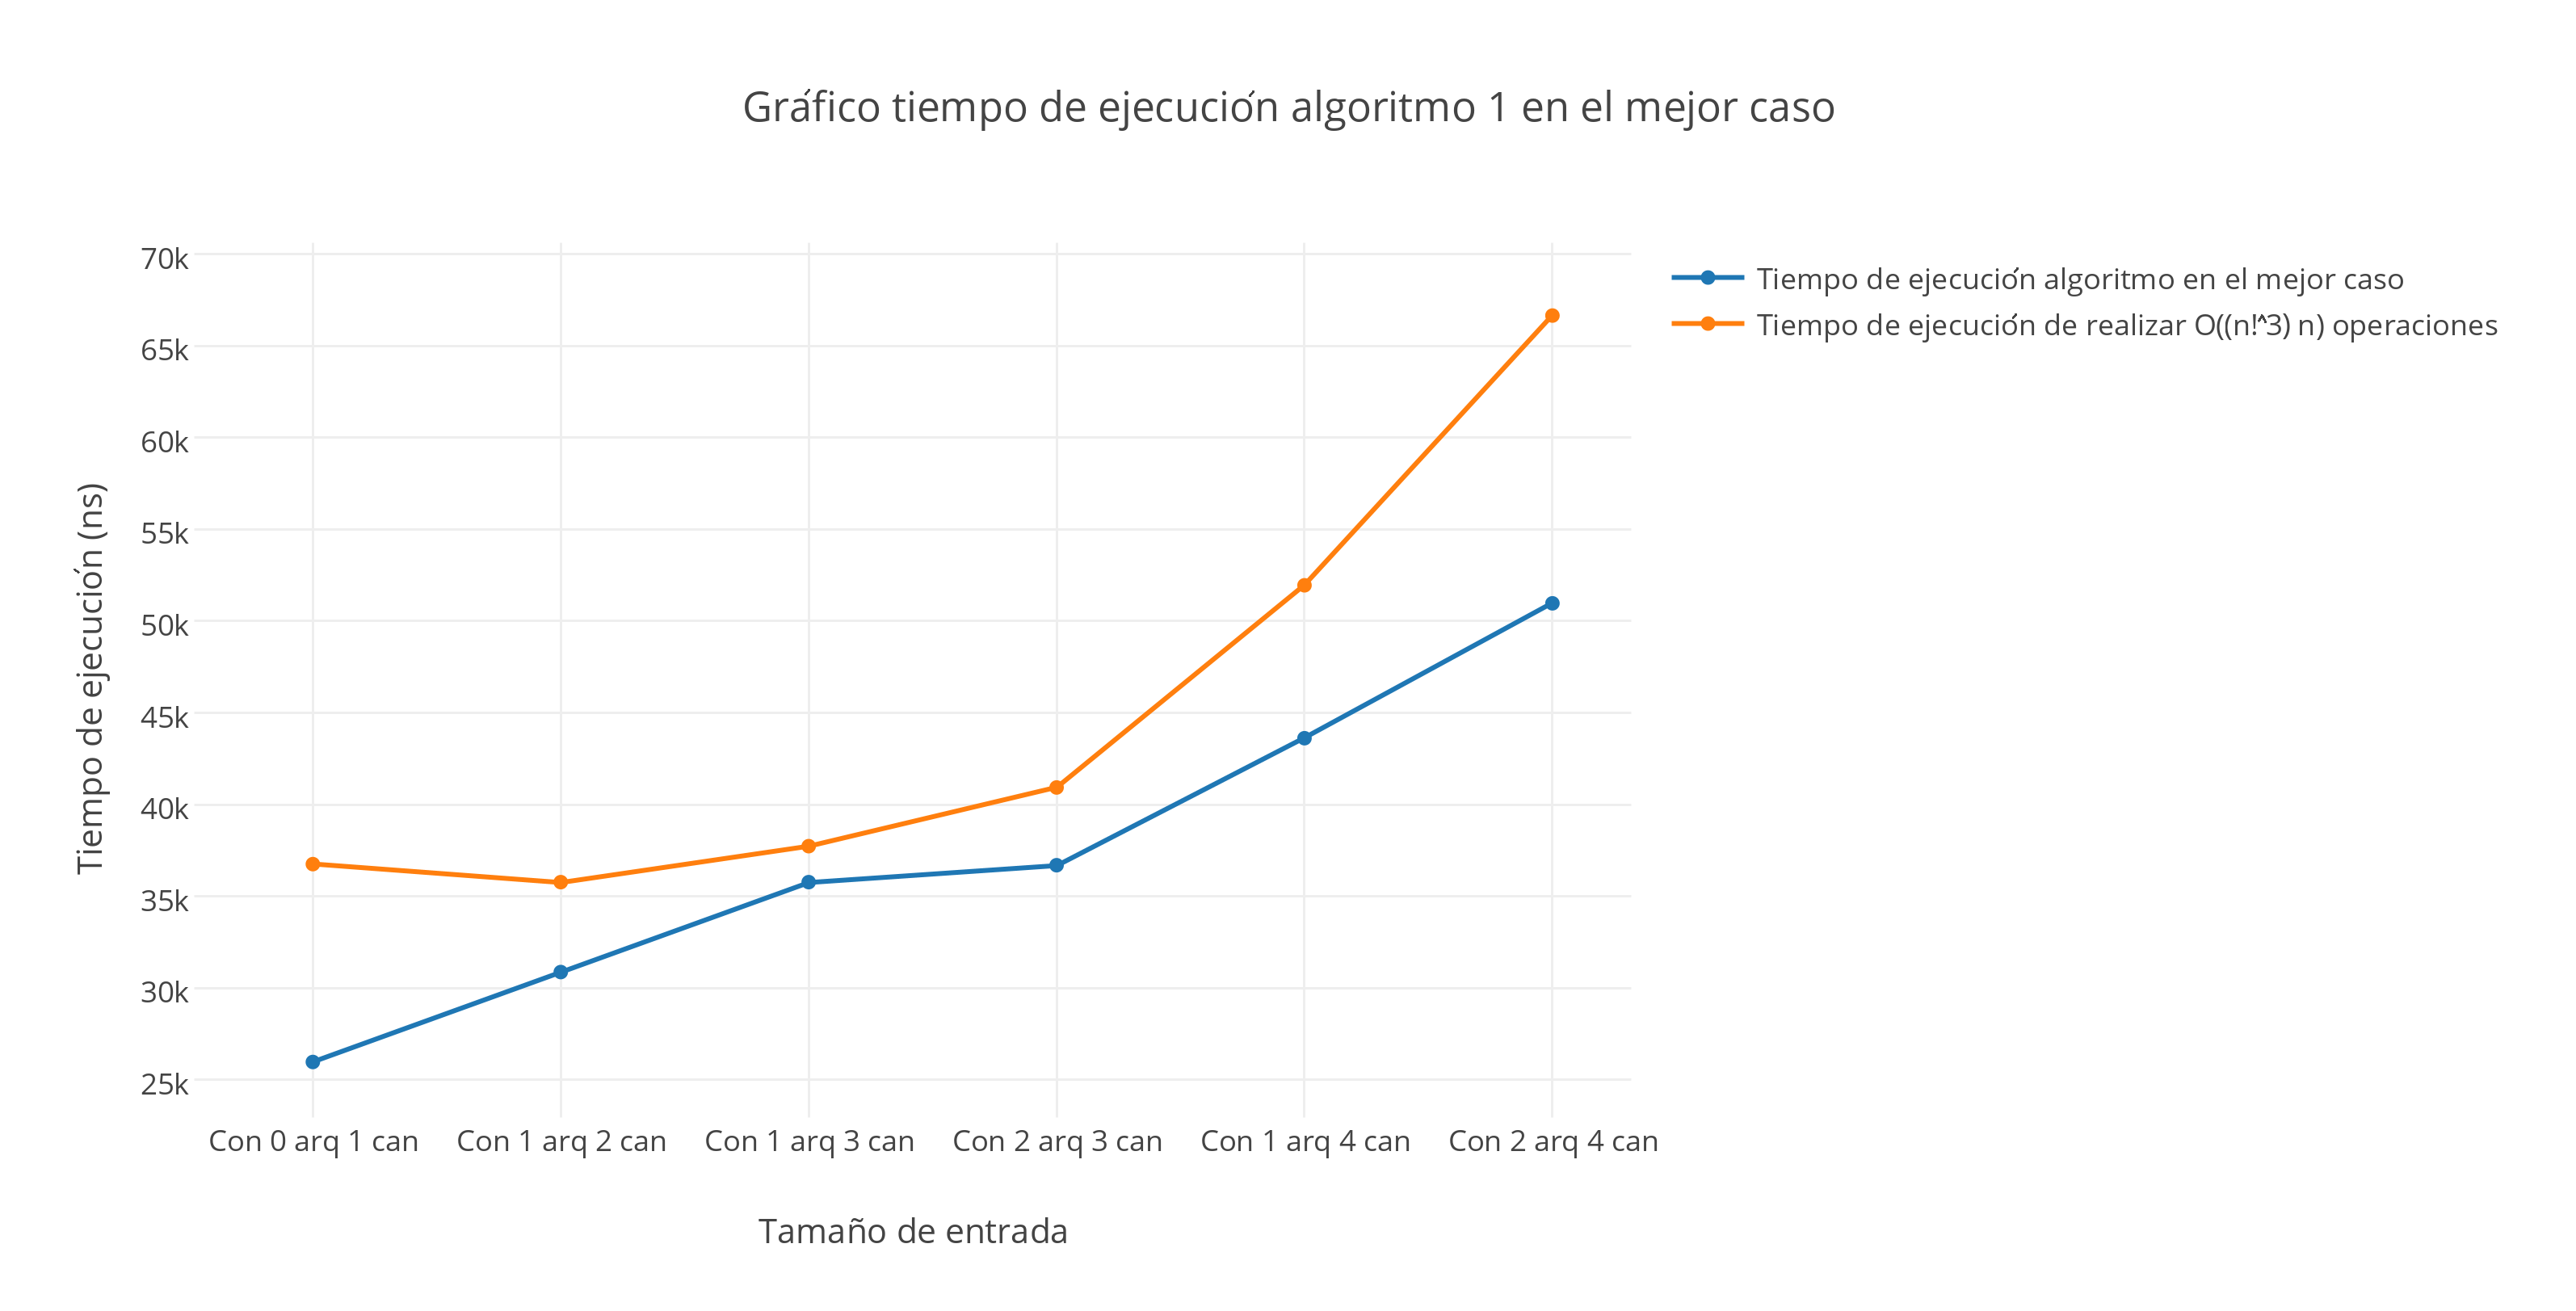
\includegraphics[scale=0.65]{./EJ1/mejorcasoej1.png}
 {$Gr$\'a$fico$ \ 1.1 - $Mejor$ $Caso$}
  \end{center}
  \vspace*{0.3cm}


Si a esto lo dividimos por la complejidad propuesta obtenemos:\\

\vspace*{0.3cm} \vspace*{0.3cm}
  \begin{center}
 %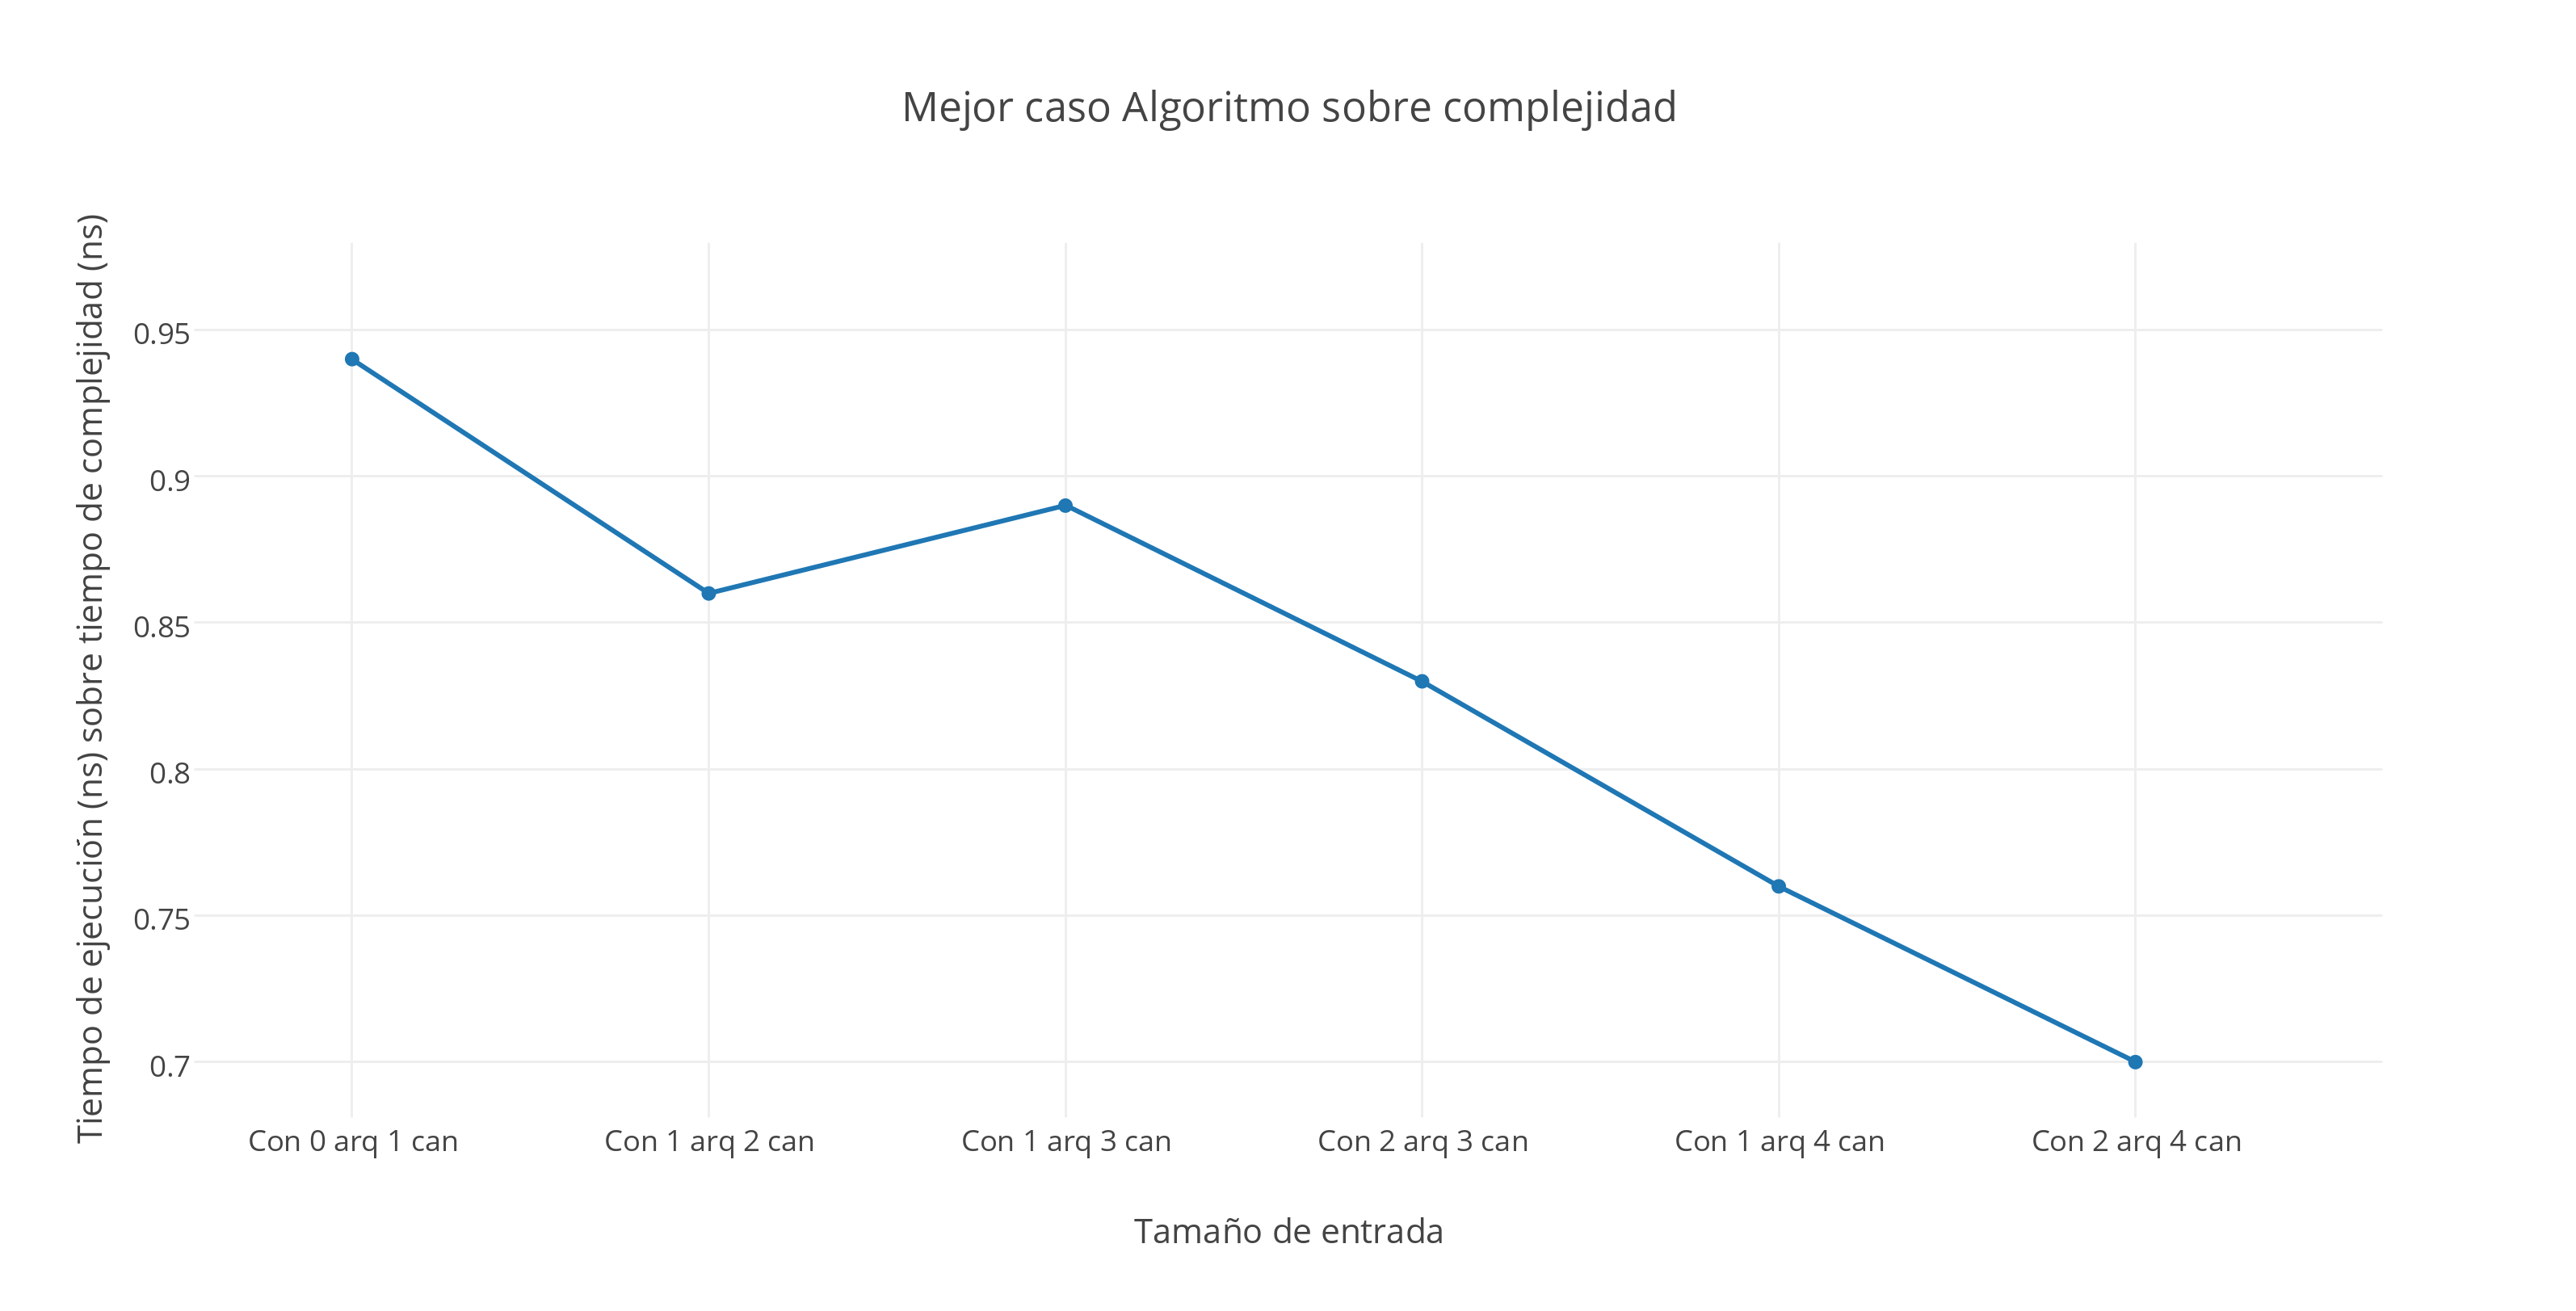
\includegraphics[scale=0.65]{./EJ1/mejorcasoej11.png}
 {$Gr$\'a$fico$ \ 1.2 - $Mejor$ $Caso$ / $Complejidad$}
  \end{center}
  \vspace*{0.3cm}

 Para realizar esta divisi\'on realizamos un promedio con el mismo input de aproximadamente 20 corridas tanto para la complejidad como para nuestro algoritmo y una vez calculado dicho promedio de ambas cosas realizamos la divisi\'on para
obtener resultados m\'as consisos.\\ 

Luego de realizar dicha divisi\'on, el promedio de dichos valores resultante fue el siguiente:

\begin{center}
\begin{table}[H]

    \begin{tabular}{ | l |l |}
    \hline

\textbf{Promedio} & 0.83 \\ \hline

    \end{tabular}
\end{table}
\end{center}


Se puede observar en la figura 1.2 que luego de realizar la divisi\'on de los tiempos la funcion resultante permanece siempre por debajo de 1 lo cual corrobora para el mejor caso que el mismo se encuentra correctamente acotado por la complejidad calculada anteriormente.\\

Luego, uno de los peores casos para nuestro algoritmo es en el cual tanto \textbf{se debe recorrer todos los posibles caminos ya que son todos exactamente iguales}, esto se da as\'i ya que nuestro algoritmo chequea todos los caminos posibles y como todos pueden ser soluci\'on posible avanza por todos y llega al final del laberinto con el mismo valor en todos los posibles caminos\\

\vspace*{0.3cm} \vspace*{0.3cm}
  \begin{center}
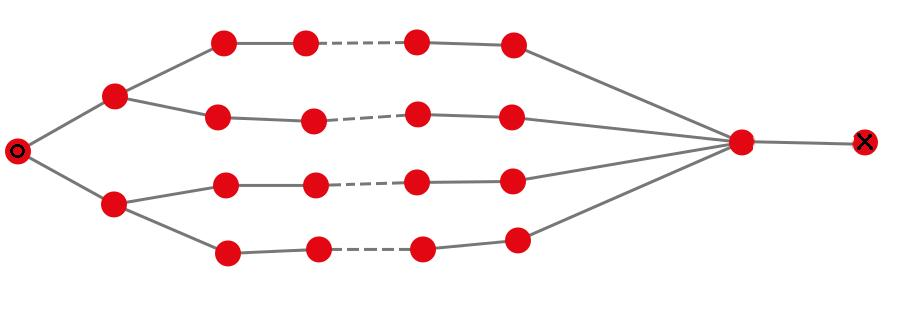
\includegraphics[scale=0.65]{./EJ1/ej1grafopeorcaso.jpeg}
{$Ejemplo Grafo$ \ 1.2 - $Peor$ $Caso$}
  \end{center}
  \vspace*{0.3cm}


\vspace*{0.3cm} \vspace*{0.3cm}
  \begin{center}
%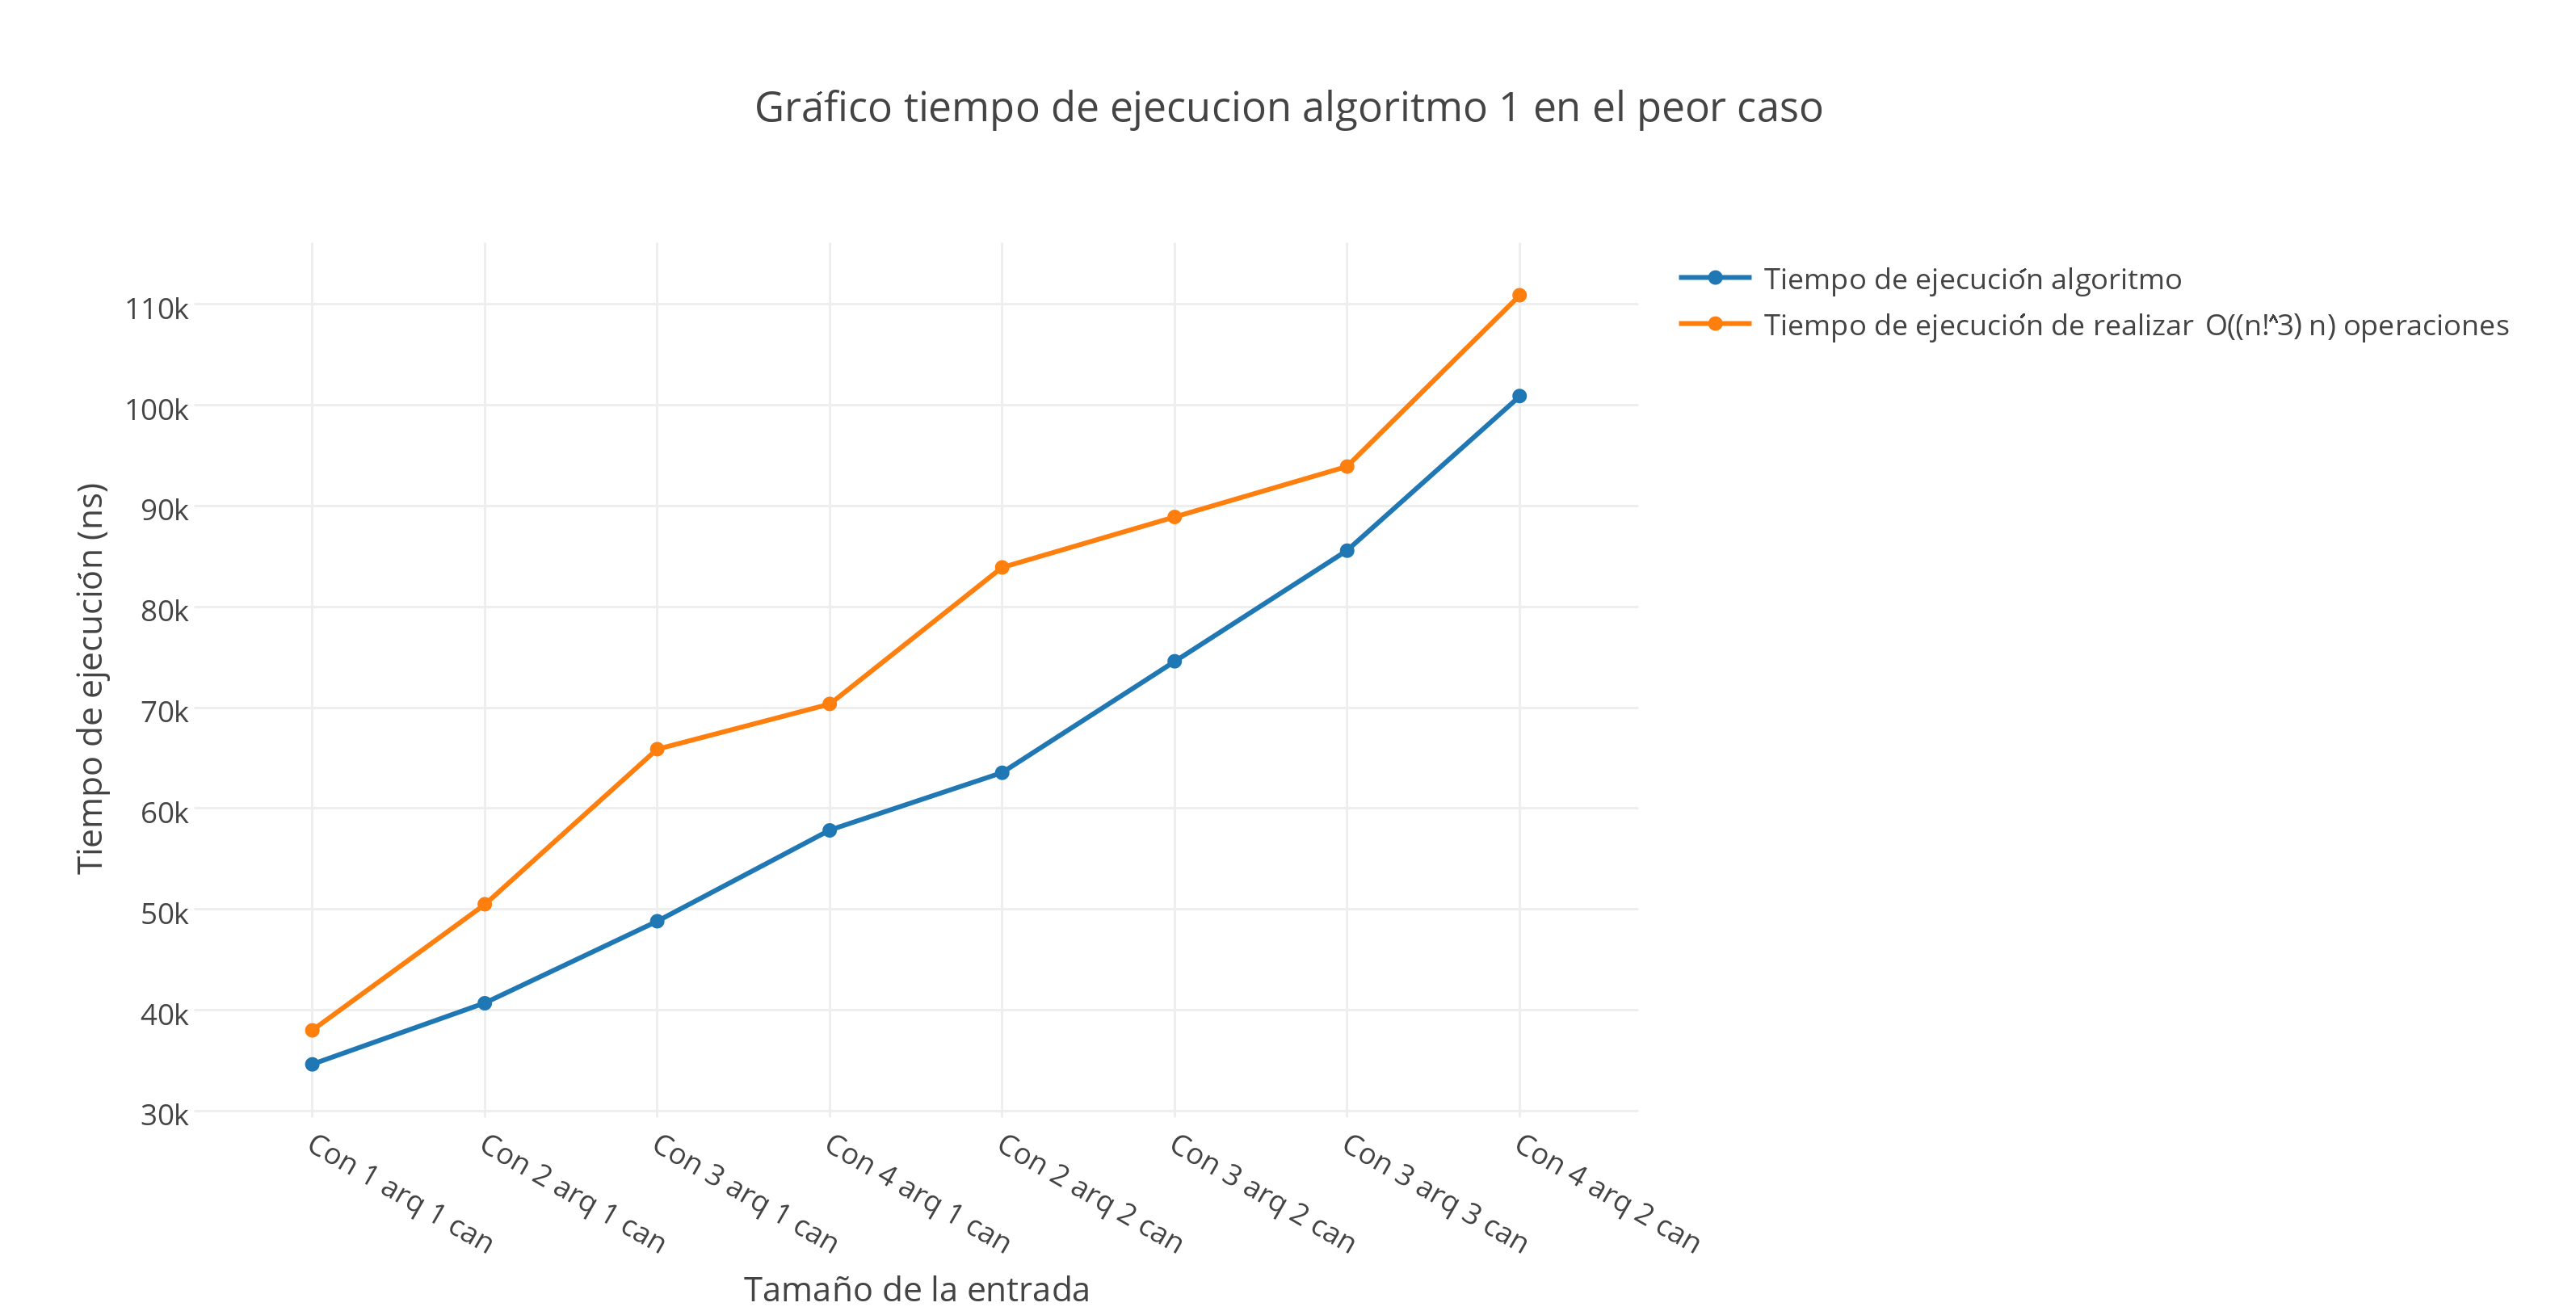
\includegraphics[scale=0.65]{./EJ1/peorcasoej1.png}
{$Gr$\'a$fico$ \ 1.3 - $Peor$ $Caso$}
  \end{center}
  \vspace*{0.3cm}

Si a esto lo dividimos por la complejidad propuesta obtenemos:\\

\vspace*{0.3cm} \vspace*{0.3cm}
  \begin{center}
% 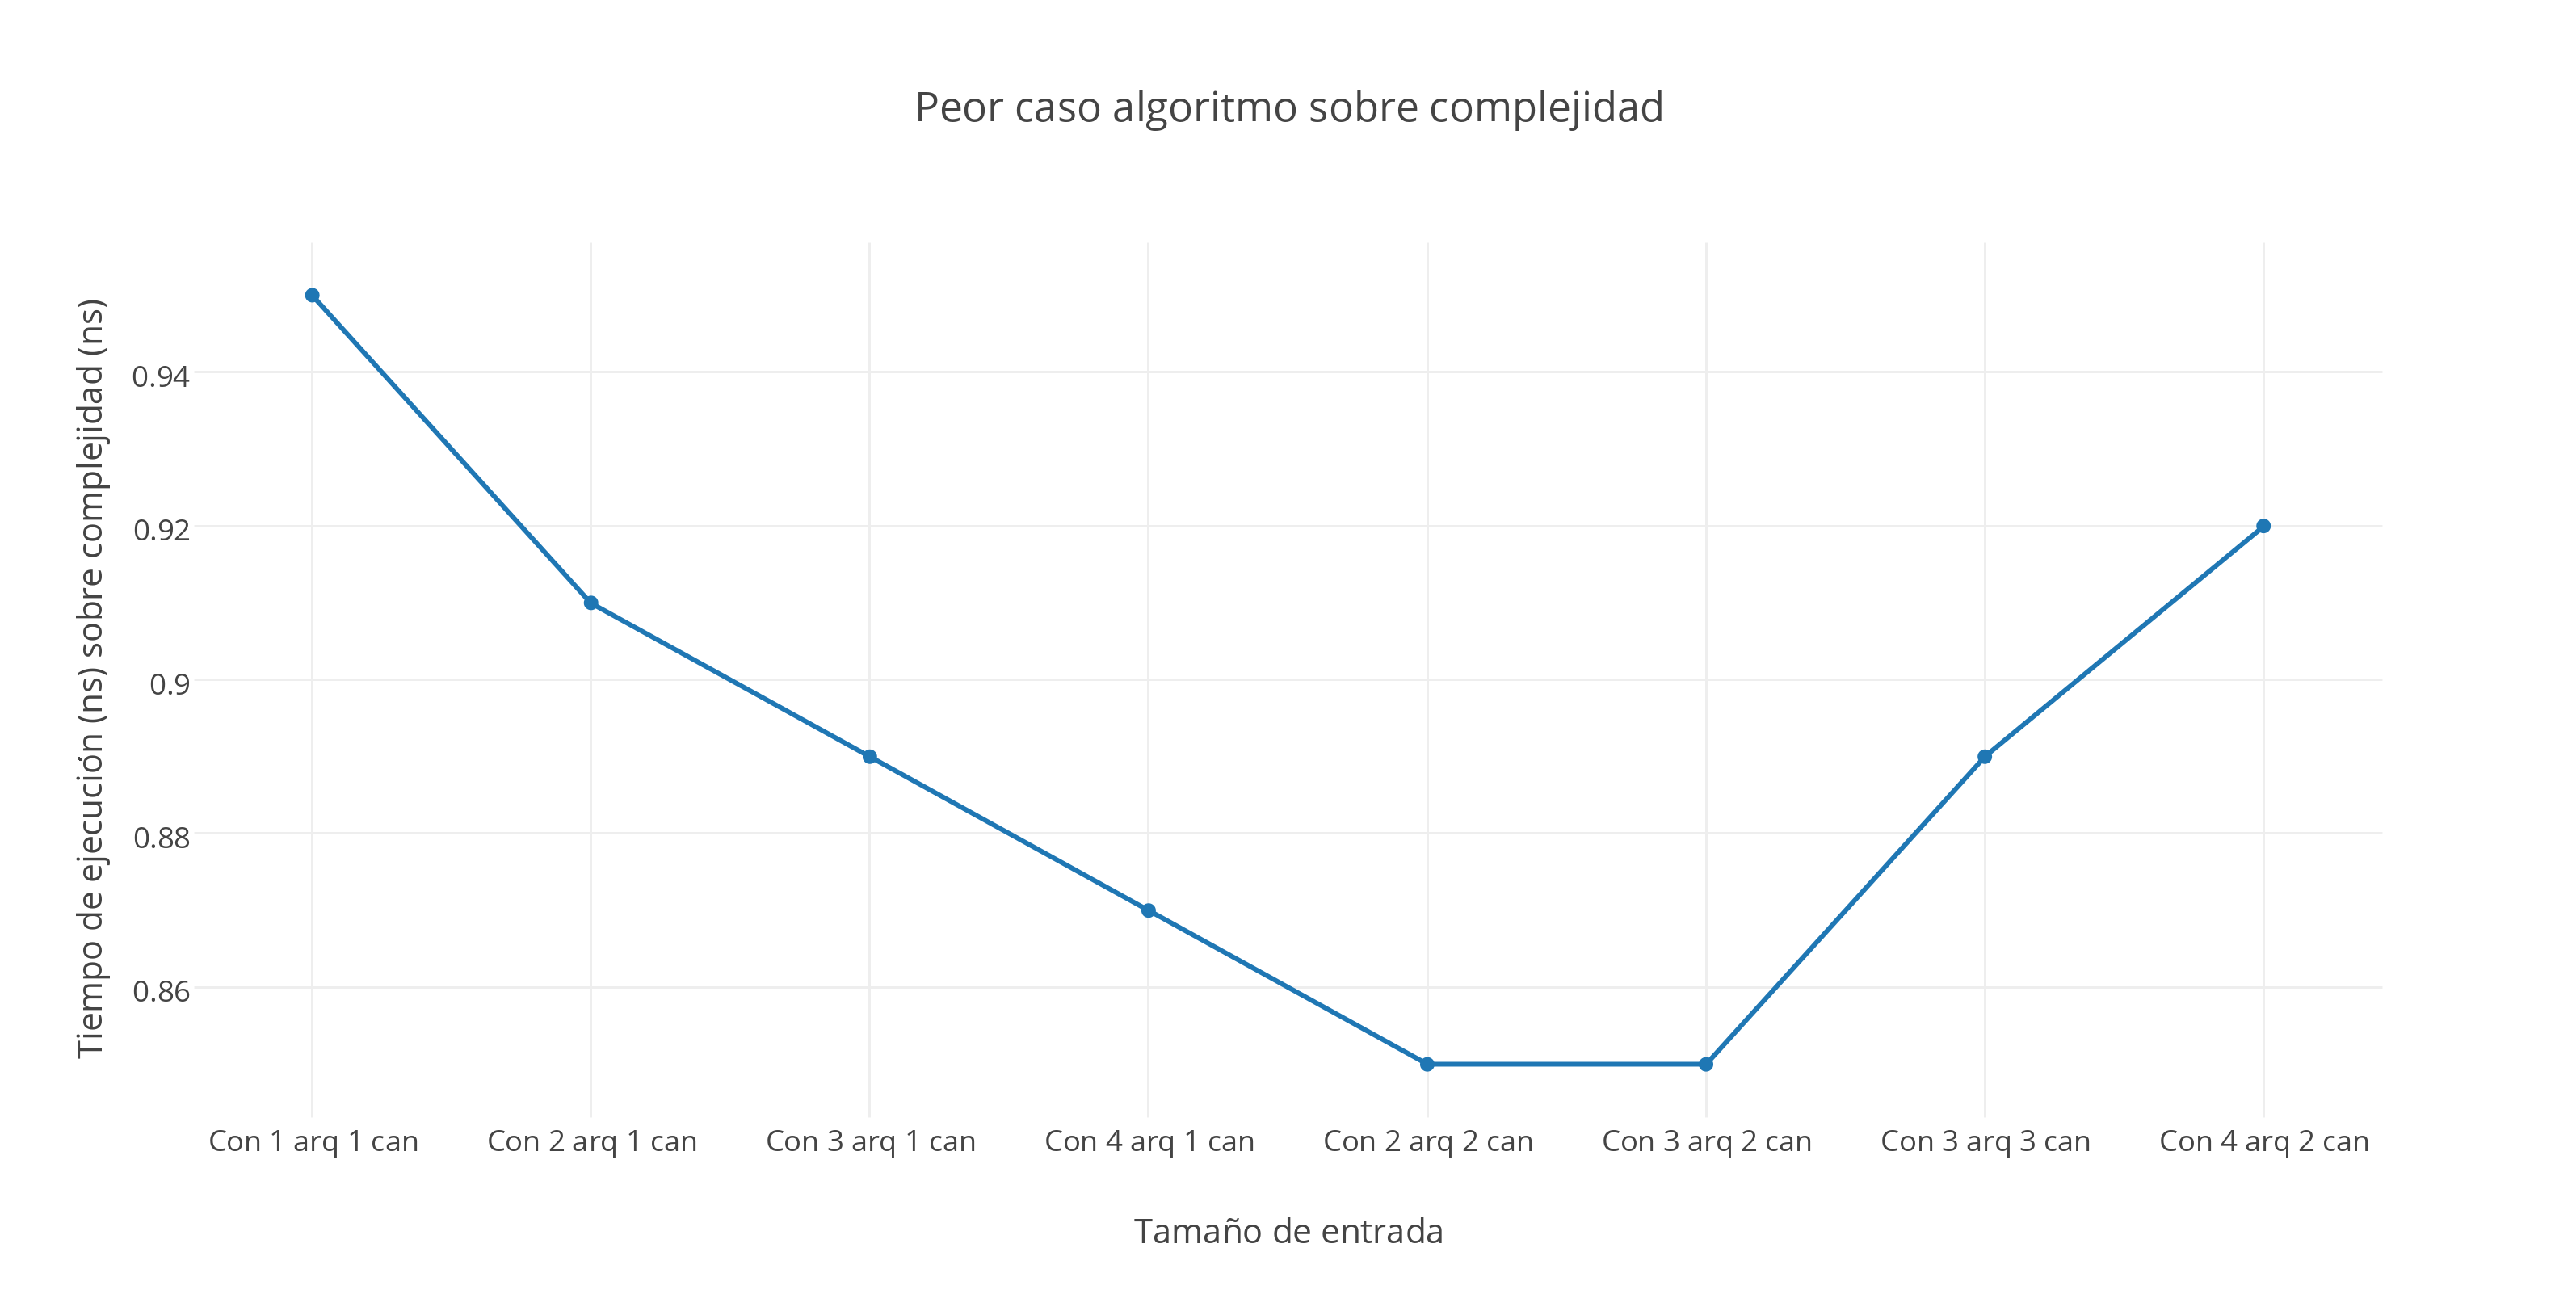
\includegraphics[scale=0.65]{./EJ1/peorcasoej11.png}
 {$Gr$\'a$fico$ \ 1.4 - $Peor$ $Caso$ / $Complejidad$}
  \end{center}
   \vspace*{0.3cm}
  
  Para realizar esta experimentaci\'on nos parecio acorde, realizar un promedio con el mismo input de aproximadamente 20 corridas tanto para la complejidad como para nuestro algoritmo y una vez calculado dicho promedio de ambas cosas realizamos la divisi\'on para obtener resultados m\'as relevantes.\\ 

Luego de realizar dicha divisi\'on, el promedio de dichos valores resultante fue el siguiente:

\begin{center}
\begin{table}[H]
    \begin{tabular}{ | l |l |}
    \hline
	
    \textbf{Promedio} &  0.89 \\ \hline

    \end{tabular}
\end{table}
\end{center}

Podemos observar en la figura 1.4 como la funci\'on resultante se mantiene por debajo de 1, a pesar de tener casos en los cuales la funci\'on llega a un m\'inimo el cual se encuentra muy por debajo de 1, lo cual se da por la implementaci\'on del algoritmo.\\

Luego de lo mostrado, podemos ver que ya sea en el peor caso nuestro algoritmo en funci\'on al tiempo de ejecuci\'on queda asintotizado por debajo de la funci\'on del tiempo de la complejidad .